\documentclass[conference]{IEEEtran}

\usepackage[utf8]{inputenc}
\usepackage[T1]{fontenc}
\usepackage{amsmath,amssymb,amsfonts,bm}
\usepackage{graphicx}
\graphicspath{{figures/}{./}}
\usepackage{booktabs}
\usepackage{array}
\usepackage{balance}
\usepackage{enumitem}
\usepackage{cite}
\usepackage{url}
\usepackage[hidelinks]{hyperref}
\usepackage{tikz}
\usetikzlibrary{arrows.meta,positioning,fit,calc}
\usetikzlibrary{arrows.meta,positioning,fit}
\usepackage[utf8]{inputenc}
\usepackage[T1]{fontenc}
\usepackage{amsmath,amssymb,amsthm}
\usepackage{booktabs,array,multirow}
\usepackage{placeins}
\usepackage{graphicx}
\usepackage{xcolor}
\usepackage{tikz}
\usetikzlibrary{arrows.meta,positioning,fit,calc}
\usepackage[hidelinks]{hyperref}
\newcommand{\prism}{PRISM-XAI}
\newcommand{\mapx}{MAP-XAI}
\newtheorem{theorem}{Theorem}
\newtheorem{proposition}{Proposition}
\newcommand{\method}{PRISM-XAI}
\newcommand{\mapxai}{MAP-XAI}
\newcommand{\E}{\mathbb{E}}
\newcommand{\medmath}[1]{#1}

\begin{document}

\title{PRISM-XAI: Privacy-Accounted Semantic Explanation Scheduling for Smart-Grid Edge Intelligence}
\author{\IEEEauthorblockN{Author information available in the submission system}}

\maketitle


\begin{abstract}
In smart-grid edge monitoring, communicating
explanations from distributed endpoints introduces
wireless transmission overhead and cumulative
privacy expenditure. Scheduling these updates
therefore requires balancing communication resources,
explanation availability, and privacy constraints.
We propose a two-layer framework comprising
MAP-XAI and PRISM-XAI. MAP-XAI constructs
explanation packets by clipping attribution
changes, applying Gaussian perturbation, and
subsequently performing Top-$k$ selection and
quantization, with cumulative privacy expenditure
tracked using R\'enyi differential privacy.
PRISM-XAI selects endpoints and packet resolutions,
or abstains from transmission, using declared
public-state information on channel conditions,
explanation freshness, event criticality, forecast
novelty, and fairness, without directly accessing
private attribution values.
We evaluate the framework using OPSD and UCI
electricity datasets in a simulated wireless
uplink environment. The primary evaluation
comprises 720 runs, including 120 paired
MAP-XAI-only and PRISM-XAI comparisons.
Under predefined service-matching criteria
and comparable recorded privacy expenditure,
PRISM-XAI reduces transmitted traffic by
$15.72\%$ relative to MAP-XAI-only, with a
paired mean reduction of $36.40\pm3.32$~kbit
(95\% confidence interval half-width).
Differences in the evaluated critical-event
coverage and recall proxies are not
statistically detected, although their
absolute levels remain low. Fixed-DP baselines
operate at different service levels and are
therefore not used to establish matched-service
superiority. Top-$K$ attribution overlap exceeds
the random reference on OPSD but not on UCI,
providing dataset-dependent agreement evidence
rather than demonstrated operational explanation
utility. These results indicate that public-state
scheduling can reduce explanation traffic
relative to the packetization-only configuration
under the tested conditions. Privacy accounting
applies to released packet contents under the
stated assumptions and does not establish
privacy protection for transmission timing,
endpoint selection, or the complete communication
transcript.
\end{abstract}


\begin{IEEEkeywords}
smart-grid communications, load-forecast explanations, explainable AI,
differential privacy, explanation scheduling, resource allocation,
Age of Explanation
\end{IEEEkeywords}



\section{Introduction}
\label{sec:introduction}

Short-term electricity-load forecasting supports grid
monitoring, demand management, and operational planning.
Although machine-learning models can provide accurate
forecasts, operators may also need to understand which
inputs influence individual predictions. Explainable
artificial intelligence (XAI) methods, such as SHAP
~\cite{lundberg2017shap} and Integrated Gradients
~\cite{sundararajan2017ig}, help identify the contributions
of lagged demand, rolling statistics, and calendar
features. Recent research has examined XAI for electricity
load forecasting~\cite{baur2024loadxai} and explainable
anomaly detection in grid monitoring
~\cite{gebhard2025anomaly}. These studies demonstrate
the relevance of model explanations in energy systems.
However, identifying influential features does not
establish the physical causes of demand changes, and
generating explanations is only one part of making
them available for operational use.

In distributed grid-monitoring systems, explanations
generated at household endpoints may need to be
communicated repeatedly to an edge server or operator.
This creates three practical challenges. First,
household-level explanations may reveal sensitive
information about electricity consumption and user
behaviour~\cite{shokri2021privacy}. Second, transmitting
detailed explanations consumes wireless resources and
may introduce delays. Third, protecting each
transmission does not remove the privacy cost of
repeated releases: privacy expenditure accumulates
over time, limiting how frequently explanations can
be shared. Therefore, transmitting every explanation
is neither necessarily communication-efficient nor
compatible with a fixed long-term privacy budget.


Recent studies have addressed related challenges from
different perspectives. Federated-XAI research identifies
explanation privacy, communication overhead, and continual
explainability as important challenges
~\cite{gholizade2026fedxai}. HXAI
~\cite{sengupta2026hxai} investigates hierarchical,
privacy-preserving explainability in distributed energy
systems, motivating the need to protect explanation
information shared across system levels. Related
privacy-adaptive learning approaches examine the
balance between privacy and utility
~\cite{piran2025privatedfl,li2026fedsva}.
Meanwhile, task-oriented communication prioritizes
information according to downstream relevance
~\cite{ma2023semantic}, while recent information-freshness
research studies update scheduling under limited
transmission opportunities
~\cite{aoi2025feedback,aoi2025updates}.
However, these research directions do not directly
resolve how to schedule repeated attribution-packet
releases while jointly accounting for wireless
resources, explanation fidelity, operational deadlines,
and cumulative household privacy expenditure.



The remaining gap is the joint design of private explanation packets
and their wireless delivery. Unlike privacy-aware explanation generation
such as HXAI~\cite{sengupta2026hxai}, repeated transmission must balance
fidelity against a finite privacy allowance: frequent releases increase
coverage but may demand more noise per release. This motivates deciding
\emph{what to send, when, and when to abstain} under privacy, wireless,
and operational constraints.
In the considered edge-monitoring architecture, household endpoints share the
uplink used to update an operator's view of forecast behaviour. An explanation
update differs from conventional fixed-format telemetry: its semantic
resolution determines packet size, its value decays while the operator holds
an older explanation, and each private release consumes part of a finite
horizon budget. Consequently, communication control cannot be reduced to
choosing the endpoint with the strongest channel. It must choose both the
endpoint and explanation resolution while enforcing resource-block capacity,
fading-dependent latency, delivery deadlines, freshness, and privacy
admission. PRISM-XAI addresses precisely this cross-layer scheduling problem.

To address this gap, we contribute a two-layer framework. \mapxai{} is the
privacy-accounted representation layer: it clips attribution changes, adds
Gaussian noise, compresses the resulting private vector, and admits releases
through cumulative RDP accounting. \method{} is the resource-allocation
layer: it uses AoX, public grid criticality, channel state, endpoint fairness,
and a public forecast-novelty score to choose endpoints, modes, or abstention.
Thus MAP-XAI and PRISM-XAI are complementary contributions, and the
MAP-XAI-only configuration provides the component ablation. Specifically:
\begin{itemize}[leftmargin=*,nosep]
    \item \textbf{Two-layer co-design:} MAP-XAI provides private selective
    explanation packets; PRISM-XAI schedules them without consulting the raw
    attribution-residual norm.
    \item \textbf{Explanation-aware uplink scheduling:} the scheduler jointly
    selects household endpoints, semantic packet resolution, and abstention
    under resource-block, deadline, channel, freshness, and privacy constraints
    arising in shared smart-grid edge links.
    \item \textbf{Matched component evidence:} over 120 paired runs,
    PRISM-XAI lowers traffic by 15.72\% relative to MAP-XAI alone while
    preserving the tested coverage, recall, fairness, and privacy expenditure.
    \item \textbf{Robust evaluation:} 2,160 experiments across two datasets,
    two explanation methods, three privacy budgets, scheduler variants, and
    paired random seeds quantify traffic--service trade-offs.
\end{itemize}
Our objective is to characterize when selective,
privacy-accounted explanation delivery is feasible
and what trade-offs it introduces, rather than
to assume that reducing communication alone
improves operational performance.

The rest of the paper keeps the two contributions separate. Section II first
defines MAP-XAI's packet mechanism and privacy accountant, and then describes
the PRISM-XAI scheduler that operates on the available packet modes. Section
III explains the datasets, service metrics, matched-comparison rule, and
statistical protocol before presenting the main and sensitivity results. We
end by separating what the experiment establishes from the stronger privacy
and operational claims that remain future work.

\section{Two-Layer Private Explanation Delivery}

\subsection{System and threat model}

Let $\mathcal H=\{1,\ldots,N\}$ denote household endpoints grouped into
zones $\mathcal H_z$. At slot $t$, endpoint $i$ observes
$\bm x_{i,t}\in\mathbb R^d$, a deployed forecaster $f$ produces
$\hat y_{i,t}$, and an explainer produces
$\bm\phi_{i,t}=\mathcal E(f,\bm x_{i,t})\in\mathbb R^d$. Raw features and
non-private attributions remain local. The trusted endpoint privatizes a
packet before exposing it to the edge; the edge and operator may observe
all transmitted packet contents and scheduling outcomes. Timing
side-channels are outside the formal content-DP guarantee and require
fixed opportunities or dummy traffic in timing-sensitive deployments.

\begin{figure*}[t]
\centering
\resizebox{0.88\linewidth}{!}{%
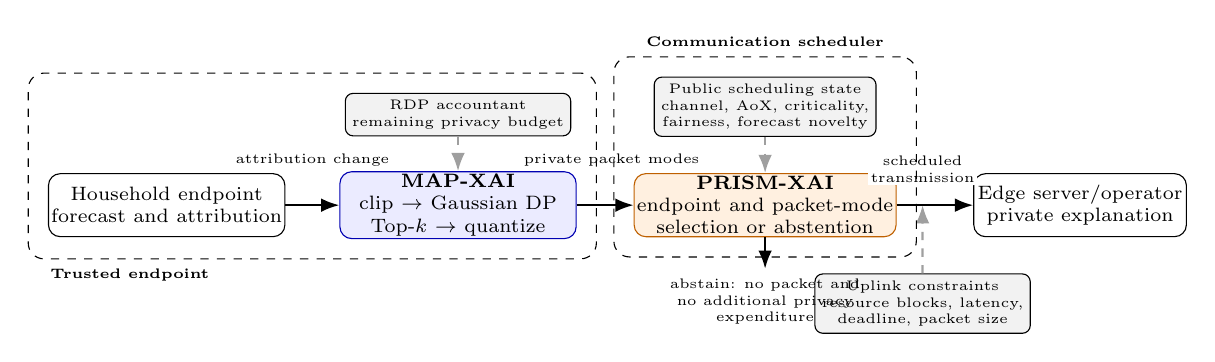
\begin{tikzpicture}[
    font=\scriptsize,
    >=Latex,
    block/.style={
        draw,
        rounded corners=1.5mm,
        align=center,
        minimum height=8mm,
        minimum width=27mm,
        inner sep=1pt
    },
    mapblock/.style={
        block,
        fill=blue!8,
        draw=blue!70!black,
        minimum width=30mm
    },
    prismblock/.style={
        block,
        fill=orange!12,
        draw=orange!75!black,
        minimum width=32mm
    },
    info/.style={
        draw,
        rounded corners=1mm,
        fill=gray!10,
        align=center,
        font=\tiny,
        inner sep=2.5pt
    },
    region/.style={
        draw,
        dashed,
        rounded corners=2mm,
        inner sep=2.5mm
    },
    flow/.style={->,thick},
    control/.style={->,dashed,thick,gray!75}
]

% Main communication path
\node[block] (endpoint) at (0,0) {
    Household endpoint\\
    forecast and attribution
};

\node[mapblock] (map) at (3.7,0) {
    \textbf{MAP-XAI}\\
    clip $\rightarrow$ Gaussian DP\\
    Top-$k$ $\rightarrow$ quantize
};

\node[prismblock] (prism) at (7.6,0) {
    \textbf{PRISM-XAI}\\
    endpoint and packet-mode\\
    selection or abstention
};

\node[block] (edge) at (11.6,0) {
    Edge server/operator\\
    private explanation
};

% Supporting inputs
\node[info] (accountant) at (3.7,1.15) {
    RDP accountant\\
    remaining privacy budget
};

\node[info] (public) at (7.6,1.25) {
    Public scheduling state\\
    channel, AoX, criticality,\\
    fairness, forecast novelty
};

\node[info] (radio) at (9.6,-1.25) {
    Uplink constraints\\
    resource blocks, latency,\\
    deadline, packet size
};

% Main arrows without long overlapping labels
\draw[flow] (endpoint) -- (map);
\draw[flow] (map) -- (prism);
\draw[flow] (prism) -- (edge);

% Control inputs
\draw[control] (accountant) -- (map);
\draw[control] (public) -- (prism);
\draw[control] (radio) -- ($(prism)!0.50!(edge)$);

% Short labels placed above arrows
\node[
    font=\tiny,
    fill=white,
    inner sep=1pt,
    above=4.5mm
] at ($(endpoint)!0.5!(map)$) {
    attribution change
};

\node[
    font=\tiny,
    fill=white,
    inner sep=1pt,
    above=4.5mm
] at ($(map)!0.5!(prism)$) {
    private packet modes
};

\node[
    font=\tiny,
    fill=white,
    inner sep=1pt,
    above=2.5mm,
    align=center
] at ($(prism)!0.5!(edge)$) {
    scheduled\\transmission
};
% Abstention path
\draw[flow] (prism.south) -- ++(0,-0.4)
    node[below,align=center,font=\tiny]
    {abstain: no packet and\\no additional privacy \\ expenditure};

% Functional boundaries
\node[
    region,
    fit=(endpoint)(map)(accountant),
    label={[font=\tiny\bfseries]below left:
        Trusted endpoint}
] {};

\node[
    region,
    fit=(prism)(public),
    label={[font=\tiny\bfseries]above:
        Communication scheduler}
] {};

\end{tikzpicture}%
}
\caption{PRISM-XAI communication architecture. MAP-XAI forms
privacy-accounted explanation-packet modes locally. PRISM-XAI uses public
grid and channel state to select an endpoint and packet resolution, or to
abstain, subject to uplink resource and deadline constraints.}
\label{fig:architecture}
\end{figure*}

Figure~\ref{fig:architecture} can be read from left to right. First, a household
computes a forecast and a local attribution vector. Second, MAP-XAI converts
the attribution change into one or more privacy-accounted packet options.
Third, PRISM-XAI sees only declared public state and the metadata of those
options; it chooses one option or abstains. Finally, the edge reconstructs the
received private explanation. MAP-XAI therefore answers ``how can an
explanation be released?'', whereas PRISM-XAI answers ``which admissible
release should use the current wireless opportunity?''

\begin{table}[t]
\caption{Separation of responsibilities in the proposed stack.}
\label{tab:roles}
\centering
\scriptsize
\setlength{\tabcolsep}{3.1pt}
\begin{tabular}{p{0.20\columnwidth}p{0.34\columnwidth}p{0.36\columnwidth}}
\toprule
Layer & Inputs used & Output and responsibility\\
\midrule
MAP-XAI & Local attribution change; clipping radius; noise, Top-$k$, and quantization settings & Private packet alternatives and their RDP costs\\
PRISM-XAI & Public forecast novelty, criticality, AoX, channel state, fairness state, and packet metadata & Endpoint, packet mode, or abstention under the slot budget\\
Accountant & Per-release noise multiplier and previous admitted releases & Admit/reject decision and cumulative privacy expenditure\\
\bottomrule
\end{tabular}
\end{table}

\subsection{MAP-XAI: privacy-protected packetization}
\begingroup
\setlength{\abovedisplayskip}{4pt}
\setlength{\belowdisplayskip}{4pt}
\setlength{\abovedisplayshortskip}{2pt}
\setlength{\belowdisplayshortskip}{2pt}

Let $t_i^-$ denote the last explanation successfully delivered to the operator before slot $t$. The endpoint forms $\Delta\bm\phi_{i,t}=\bm\phi_{i,t}-\bm\phi_{i,t_i^-}$ and clips it to $\ell_2$ radius $C_i$:
\begin{equation}
\medmath{\overline{\Delta\bm\phi}_{i,t}=
\frac{\Delta\bm\phi_{i,t}}
{\max\{1,\|\Delta\bm\phi_{i,t}\|_2/C_i\}}}.
\label{eq:clip}
\end{equation}
For an add/remove adjacency in which an absent household contributes the zero vector, a clipped contribution has sensitivity at most $C_i$. This bound applies only if the reference attribution is public, fixed, or computed entirely from previously released private outputs; otherwise its dependence on private data must also be included in the sensitivity analysis. A Gaussian mechanism then releases
\begin{equation}
\medmath{\widetilde{\Delta\bm\phi}_{i,t}=
\overline{\Delta\bm\phi}_{i,t}+\bm n_{i,t},\quad
\bm n_{i,t}\sim\mathcal N(0,\sigma_{i,t}^2\Delta_i^2\bm I_d).}
\label{eq:gauss}
\end{equation}
Only after Eq.~\eqref{eq:gauss} does \mapxai{} retain Top-$k$ coordinates and quantize their magnitudes. Hence selection and quantization are DP post-processing. A mode $m=(k,q,\sigma)$ has packet size
\begin{equation}
\medmath{S_i(m)=S_0+k(\lceil\log_2 d\rceil+q+1),}
\label{eq:size}
\end{equation}
where the final bit carries the sign. Different $k$, $q$, and $\sigma$ values define packet-resolution/privacy levels; a no-release action spends no privacy.
We account for repeated release with R\'enyi-DP (RDP)
~\cite{mironov2017rdp}. At order $\alpha$, a Gaussian release costs
$\rho_{i,t}(\alpha)=\alpha/(2\sigma_{i,t}^2)$. The endpoint composes
these costs and rejects a private release that would exceed the remaining
budget. At the end of the protected horizon,
\begin{equation}
\medmath{\epsilon_i(\delta_i)=\min_{\alpha}
\left\{\sum_t a_{i,t}\rho_{i,t}(\alpha)+
\frac{\log(1/\delta_i)}{\alpha-1}\right\}.}
\label{eq:rdp}
\end{equation}
Privacy is charged when a private packet is exposed outside the trusted
endpoint, even if it later misses the communication deadline. The
accountant must use the actual noise multiplier for every exposed release. Because
clipping fixes the sensitivity, Eq.~\eqref{eq:gauss} is Gaussian DP at
each release; Top-$k$ selection, quantization, and packet reconstruction
are post-processing. RDP composition in Eq.~\eqref{eq:rdp} therefore
provides the stated user-level horizon guarantee whenever every admitted
release remains inside the tracked RDP budget.

\paragraph{Content-privacy guarantee.}
Under the stipulated add/remove contribution adjacency (not arbitrary replacement of an endpoint's entire raw history), each exposed noisy delta
has order-$\alpha$ RDP cost $\rho_{i,t}(\alpha)=\alpha/(2\sigma_{i,t}^2)$.
Adaptive RDP composition is additive for mechanisms satisfying the stated
conditional sensitivity and noise assumptions. Subject to this conditional sensitivity bound and correct accounting, the resulting packet-content
transcript satisfies $(\epsilon_i(\delta_i),\delta_i)$-DP if the
accountant enforces the chosen horizon budget at every release.
Top-$k$ selection, quantization, reconstruction, and controller operations
that depend only on public state and previously released private outputs
are post-processing. This guarantee is for released content; an independent
timing side channel remains outside the threat model stated above.

\endgroup
\vspace{-3mm}
\subsection{PRISM-XAI: privacy-accounted scheduling}
\begingroup
\setlength{\abovedisplayskip}{4pt}
\setlength{\belowdisplayskip}{4pt}
\setlength{\abovedisplayshortskip}{2pt}
\setlength{\belowdisplayshortskip}{2pt}
Let $A_{i,t}$ be AoX and $w^{\rm crit}_{i,t}\geq 1$ a public
criticality weight. A candidate mode must fit the available resource
blocks, meet the $D_i^{\max}$ deadline, and pass RDP admission. The
controller estimates $G_{i,t}(m)$, the expected reduction in explanation
loss, from AoX, public criticality, channel state, mode resolution, remaining
budget, and forecast novelty; it never uses the raw attribution residual or a
non-private explanation oracle for candidate selection. Forecast novelty is
scaled by the calibrated clipping norm and the candidate DP-noise floor, so a
private release is considered only when this declared public score is large
enough relative to the expected perturbation.
For a feasible mode, define gain per transmitted bit
\begin{equation}
\medmath{\Gamma_{i,t}(m)=\frac{G_{i,t}(m)}{S_i(m)}.}
\label{eq:gainbit}
\end{equation}
The nonzero candidate set includes a \mapxai{} packet mode, optional
higher-resolution modes, and a coarse zonal mode; zero transmission is
always available. A richer mode replaces the \mapxai{} mode only when
its gain per bit exceeds the \mapxai{} value by a configured margin. The
slot utility also rewards criticality-weighted AoX and under-served
endpoints while penalizing energy and RDP shadow price. The resulting
multiple-choice knapsack selects at most one mode per endpoint under the
slot resource-block limit. A minimum critical-event coverage target and
minimum Jain fairness are evaluated as service guardrails; their
reported satisfaction is empirical rather than a universal guarantee. This structure
makes \mapxai{} the privacy-accounted packetization layer and \method{} the
resource-allocation layer above it. With $M$ candidate modes per endpoint
and $B$ available resource blocks, the slot-level multiple-choice knapsack
can be solved by dynamic programming in $O(NMB)$ time; in our experiments
$M$ and $B$ are small constants. The stated $O(NMB)$ bound covers only the integer-budget knapsack
core, not gain estimation, mode feasibility, or cross-slot state updates.
The online decision does not require a non-private oracle at the edge.

\paragraph{Slot-level operation.}
At the beginning of a slot, every endpoint updates its AoX and the controller
forms public criticality and channel features. MAP-XAI enumerates packet modes
whose projected RDP charge fits the endpoint's remaining budget. PRISM-XAI
removes modes that cannot meet the deadline or resource-block constraint,
scores the surviving modes using Eq.~\eqref{eq:gainbit}, and solves the
multiple-choice knapsack. An endpoint with no selected mode remains silent and
spends no additional content-privacy budget. For a selected endpoint, privacy
is charged when the protected packet is exposed outside the trusted endpoint,
not only when delivery succeeds. The receiver updates its stored explanation
and resets AoX only after successful delivery. This ordering prevents a failed
radio transmission from being treated as either a free privacy trial or a
successful freshness update.

\paragraph{Transmission Abstention Mechanism.}
The scheduler is not required to send a low-value packet merely because a
resource block is idle. A release can be infeasible because its privacy charge
exceeds the remaining allowance, because its expected latency misses the
deadline, or because its public expected gain is too small relative to packet
size. In each case abstention preserves resources for later slots. This is the
main conceptual difference from a periodic private sender; its benefit is
evaluated only against MAP-XAI-only at a matched service point.

\endgroup
\vspace{-2mm}
\section{Evaluation Protocol, Result, and Discussion}

\subsection{Data, wireless setting, and baselines}

We use Open Power System Data (OPSD) household data and UCI
ElectricityLoadDiagrams20112014~\cite{opsd2020household,uci2015eld}.
Nine OPSD endpoints are grouped into three synthetic zones and 32 UCI
endpoints into four synthetic zones. Each forecaster uses 12 lag,
rolling-statistic, and calendar features. The tree model obtains
RMSE/MAE $0.926/0.545$ on OPSD and $1.289/0.221$ on UCI. We evaluate two
attribution implementations, TreeSHAP and feature ablation, to ensure the
scheduler conclusions can be examined across two attribution implementations.
The uplink abstraction uses eight 180~kHz resource blocks, 1~ms slots,
5~ms deadlines, 3.5~GHz carrier frequency, path loss, correlated
shadowing, small-scale fading, edge delay, and bursty failures inspired
by 3GPP TR~38.901~\cite{3gpp38901}. It is a reproducible
scheduler-level stress trace, not a link-level field validation.
For the operational proxy, a zone is critical if its public predicted
load exceeds its zone-specific calibration 80th percentile or its
absolute forecast ramp exceeds the 90th percentile. A critical event is
covered when zone-mean AoX is at most eight slots and its mean public
quality certificate is at least 0.10. The dominant explanation driver
is the largest absolute-attribution sum across four fixed feature groups;
critical-event recall counts correctly identified drivers over all
critical events. These are simulated decision proxies, not verified
physical grid interventions.

Each matrix uses $512$ evaluation slots after $96$ calibration slots,
$\epsilon_{\max}\in\{8,16,32\}$, $\delta=10^{-5}$, a 5\% coverage target,
and 0.88 minimum Jain fairness. The primary public-score M8 matrix contains
$2$ datasets $\times$ $2$ XAI methods $\times$ $3$ budgets $\times$ $6$
schedulers $\times$ $10$ paired seeds $=720$ runs. We repeat the full matrix
for a residual-score M8 variant and an M4 release-cap sensitivity, yielding
2,160 experiments in total.
External baselines are periodic fixed-DP, channel-aware fixed-DP,
AoX-aware fixed-DP, and joint scheduling with full, uncompressed private
packets. We additionally report \emph{MAP-XAI-only}, which is not an
external baseline: it restricts our stack to the \mapxai{} packet mode
and therefore isolates the incremental effect of full PRISM scheduling.
Metrics include transmitted traffic, Top-$K$ and cosine agreement,
critical-event coverage and recall, intervention precision, false
intervention, bits per correct intervention, deadline misses, Jain
fairness, and spent privacy.

\begin{table}[t]
\caption{Experimental protocol and interpretation of the primary metrics.}
\label{tab:protocol}
\centering
\scriptsize
\setlength{\tabcolsep}{3pt}
\begin{tabular}{p{0.28\columnwidth}p{0.62\columnwidth}}
\toprule
Item & Definition used in the evaluation\\
\midrule
Unit of pairing & Same dataset, XAI method, privacy budget, and random seed\\
Primary contrast & Public-score PRISM-XAI minus MAP-XAI-only\\
Traffic & Total transmitted packet bits divided by $10^3$\\
Coverage & Fraction of critical events meeting both AoX and public-quality thresholds\\
Critical recall & Correctly identified dominant drivers divided by all critical events\\
Top-$K$ fidelity & Overlap between private and non-private selected features\\
Matched region & Coverage and recall gaps $\leq0.02$; relative spent-$\epsilon$ gap $\leq5\%$\\
Multiplicity & Benjamini--Hochberg correction within each comparison family\\
\bottomrule
\end{tabular}
\end{table}

Coverage and recall are deliberately distinct. Coverage asks whether a usable
explanation was available when a critical event occurred. Recall is stricter:
an event counts only when the explanation was available and its dominant
feature group agreed with the reference. A method can therefore save traffic
by abstaining, but that choice remains visible in both service metrics.
Top-$K$ overlap is a fidelity diagnostic, not proof that an explanation helps
an operator make a better decision.

\subsection{Statistical analysis and Feasibility diagnostics}

All headline differences use paired seeds so that both methods experience the
same dataset, attribution implementation, privacy budget, and stochastic
trace. We report the paired mean difference with a 95\% confidence-interval
half-width and compute both a paired $t$-test and a Wilcoxon signed-rank test.
Benjamini--Hochberg adjustment is applied within each declared comparison
family. Statistical significance does not replace the matched-region rule: a
traffic comparison is called matched only when service and recorded privacy
expenditure also satisfy Table~\ref{tab:protocol}.
Three scheduler configurations isolate the source of the traffic reduction:
residual-score scheduling with $M=8$, the same score with a stricter $M=4$
release cap, and public-score scheduling with $M=8$. The last configuration is
the primary method; the other two are sensitivity analyses.

A separate three-seed feasibility ladder at $\epsilon_{\max}=4$ removes
one transformation at a time: (A) oracle explanation, (B) clipping only,
(C) clipping plus cumulative Gaussian DP with a full packet, and (D) DP
plus attribution compression. A release sweep then varies
$\epsilon\in\{2,4,8,16,32\}$ and the maximum private releases per
endpoint $M\in\{4,8,16,32,64\}$. These diagnostics are not used to tune
the reported 720-run matrix; they identify the mechanism that limits
explanation utility.

\subsection{Results}

\subsubsection{MAP-XAI and PRISM-XAI Comparison}
MAP-XAI and PRISM-XAI are the two proposed layers, not competing external
methods. We therefore use MAP-XAI-only to measure the incremental effect of
resource-aware endpoint/mode selection. It is the only comparator satisfying
our declared matched-region rule in all 12 dataset/XAI/privacy conditions:
absolute coverage and recall gaps at most 0.02 and relative actual-$\epsilon$
gap at most 5\%. The public-score PRISM controller transmits 207.31 kbit on
average versus 243.71 kbit for MAP-XAI-only. Across 120 seed-matched runs the
difference is $-36.40\pm3.32$ kbit (95\% CI), a 15.72\% reduction after
Benjamini--Hochberg correction ($q<10^{-40}$). Coverage changes by $-0.01$
percentage points and critical-event recall by $-0.08$ points; neither is
statistically detected. Both spend the same recorded privacy budget.
Table~\ref{tab:dataset} disaggregates the primary comparison by dataset. The
same qualitative pattern appears in both cases: PRISM-XAI sends fewer bits,
while coverage, recall, and maximum spent privacy remain nearly unchanged.
The absolute traffic level is higher on UCI because the experiment contains
more endpoints. The table is descriptive; the paired, multiplicity-adjusted
test over all 120 matched runs remains the inferential basis for the headline
claim.

A nine-point public-score sweep varies the release threshold and per-endpoint
cap. It exposes a communication--service frontier: PRISM-XAI traffic rises
from 205.41--208.83~kbit at $M=8$ to 574.63--584.33~kbit at $M=32$, while
coverage rises from 0.044--0.078 to 0.140--0.206. PRISM-XAI uses less traffic
than MAP-XAI-only throughout, but all-cell service matching holds only at
$M=8$; Supplementary Sec.~VIII provides the complete paired statistics,
condition tables, and aggregate/OPSD/UCI figures.
\begin{table}[t]
\caption{Primary MAP-XAI-only and PRISM-XAI results by dataset (60 runs per row).}
\label{tab:dataset}
\centering
\scriptsize
\setlength{\tabcolsep}{2.5pt}
\resizebox{\columnwidth}{!}{%
\begin{tabular}{llrrrrr}
\toprule
Data & Method & kbit & Top-$K$ & Coverage & Recall & $\epsilon_{\max}$\\
\midrule
OPSD & MAP-only & 106.15 & .302 & .0708 & .0330 & 18.21\\
OPSD & PRISM & \textbf{87.98} & .294 & .0710 & .0324 & 18.21\\
UCI & MAP-only & 381.26 & .229 & .0851 & .0417 & 18.21\\
UCI & PRISM & \textbf{326.63} & .245 & .0848 & .0407 & 18.21\\
\bottomrule
\end{tabular}}
\end{table}

\begin{table}[t]
\caption{Communication overhead, explanation
agreement, and service metrics across evaluated
methods (120 runs per method). External baselines
operate at different service levels.}
\label{tab:main}
\centering
\scriptsize
\setlength{\tabcolsep}{2.7pt}
\resizebox{\columnwidth}{!}{%
\begin{tabular}{lccccc}
\toprule
Method & Traffic & Top-$K$ & Coverage & Recall &
$\epsilon_{\rm spent}^{\max}$\\
 & (kbit) & & & & \\
\midrule
Periodic fixed-DP & 4645.2 & 0.252 & 0.383 & 0.178 & 10.62\\
Channel fixed-DP & 4573.8 & 0.264 & 0.334 & 0.161 & 13.85\\
AoX fixed-DP & 4643.6 & 0.255 & 0.875 & 0.386 & 10.82\\
Joint full packet & 1355.0 & 0.247 & 0.196 & 0.085 & 18.66\\
\midrule
\mapxai{}-only (ours) & 243.7 & 0.265 & 0.078 & 0.037 & 18.21\\
\method{} (ours) & \textbf{207.3} & 0.269 & 0.078 & 0.037 & 18.21\\
\bottomrule
\end{tabular}}
\end{table}


\begin{figure}[t]
\centering
\resizebox{\columnwidth}{!}{%
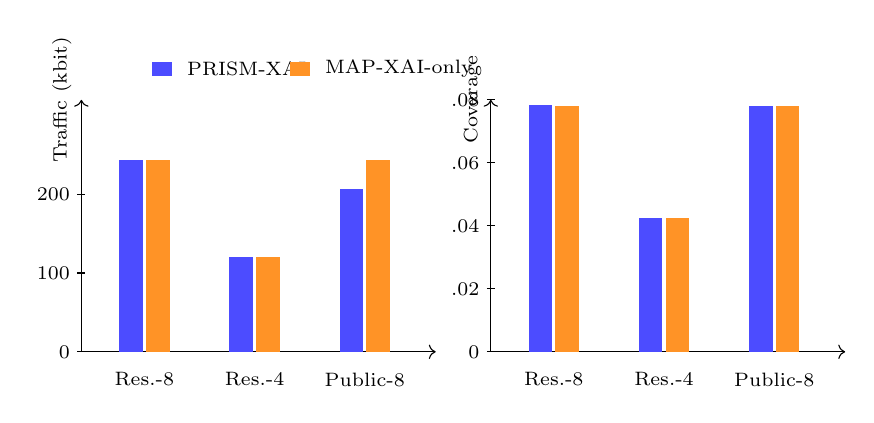
\begin{tikzpicture}[font=\scriptsize]
% Traffic panel
\draw[->] (0,0) -- (4.5,0);
\draw[->] (0,0) -- (0,3.2) node[above,rotate=90,anchor=south]{Traffic (kbit)};
\foreach \y/\lab in {0/0,1/100,2/200} {\draw (-.05,\y) -- (.05,\y) node[left=2pt]{\lab};}
\foreach \x/\lab in {.8/{Res.-8},2.2/{Res.-4},3.6/{Public-8}} {\node at (\x,-.35) {\lab};}
\fill[blue!70] (.48,0) rectangle (.78,2.43); \fill[orange!85] (.82,0) rectangle (1.12,2.44);
\fill[blue!70] (1.88,0) rectangle (2.18,1.21); \fill[orange!85] (2.22,0) rectangle (2.52,1.21);
\fill[blue!70] (3.28,0) rectangle (3.58,2.07); \fill[orange!85] (3.62,0) rectangle (3.92,2.44);
% Coverage panel
\begin{scope}[xshift=5.2cm]
\draw[->] (0,0) -- (4.5,0);
\draw[->] (0,0) -- (0,3.2) node[above,rotate=90,anchor=south]{Coverage};
\foreach \y/\lab in {0/0,.8/.02,1.6/.04,2.4/.06,3.2/.08} {\draw (-.05,\y) -- (.05,\y) node[left=2pt]{\lab};}
\foreach \x/\lab in {.8/{Res.-8},2.2/{Res.-4},3.6/{Public-8}} {\node at (\x,-.35) {\lab};}
\fill[blue!70] (.48,0) rectangle (.78,3.13); \fill[orange!85] (.82,0) rectangle (1.12,3.12);
\fill[blue!70] (1.88,0) rectangle (2.18,1.70); \fill[orange!85] (2.22,0) rectangle (2.52,1.70);
\fill[blue!70] (3.28,0) rectangle (3.58,3.12); \fill[orange!85] (3.62,0) rectangle (3.92,3.12);
\end{scope}
\fill[blue!70] (.9,3.5) rectangle (1.15,3.68); \node[anchor=west] at (1.22,3.59) {PRISM-XAI};
\fill[orange!85] (2.65,3.5) rectangle (2.90,3.68); \node[anchor=west] at (2.97,3.59) {MAP-XAI-only};
\end{tikzpicture}}
\caption{MAP-XAI-only and PRISM-XAI across residual-score M8,
residual-score M4, and public-score M8 configurations. Public-score M8
provides the primary result: lower traffic at essentially unchanged service.}
\label{fig:matched}
\end{figure}

\begin{table}[t]
\caption{Paired PRISM-XAI minus MAP-XAI-only scheduler sensitivity
($n=120$ per configuration). Coverage and recall changes are percentage points.}
\label{tab:robustness}
\centering
\scriptsize
\setlength{\tabcolsep}{2.5pt}
\resizebox{\columnwidth}{!}{%
\begin{tabular}{llrrrr}
\toprule
Score & $M$ & $\Delta$ traffic (kbit) & Relative & $\Delta$ coverage & $\Delta$ recall\\
\midrule
Residual & 8 & $-1.19\pm0.41$ & $-0.50\%$ & $+0.021$ & $-0.039$\\
Residual & 4 & $-0.02\pm0.03$ & $-0.00\%$ & $+0.002$ & $-0.136$\\
Public & 8 & $\mathbf{-36.40\pm3.32}$ & $\mathbf{-15.72\%}$ & $-0.010$ & $-0.083$\\
\bottomrule
\end{tabular}}
\end{table}


\subsubsection{External Baselines and Explanation Fidelity}

Table~\ref{tab:main} shows that MAP-XAI-only
transmits 82.0--94.8\% fewer bits than the
evaluated fixed-DP and joint full-packet baselines.
However, these methods operate at different
coverage and recall levels, so the reductions
represent communication-service trade-offs
rather than equivalent-service improvements.
PRISM-XAI further reduces transmission overhead
through adaptive scheduling.
Explanation agreement remains dataset-dependent.
On OPSD, Top-$K$ overlap exceeds the random
reference, whereas no such improvement is
detected on UCI. These results characterize
attribution agreement but do not establish
operational explanation usefulness.



\subsubsection{Interpretation of the Main Results}

The primary comparison isolates the additional
contribution of PRISM-XAI scheduling over
MAP-XAI explanation compression. Across 120
paired runs, PRISM-XAI reduces traffic from
243.71 to 207.31~kbit, corresponding to a
15.72\% reduction ($36.40\pm3.32$~kbit,
95\% confidence interval half-width).
No statistically detectable differences are
observed in critical-event coverage or recall,
and recorded privacy expenditure is unchanged.
However, the absolute coverage and recall levels
remain low, so the result supports improved
communication efficiency at the evaluated
service level rather than deployment-ready
monitoring performance.
Scheduler sensitivity analysis shows that
public-state scheduling produces greater traffic
savings than residual-score scheduling or
stricter release limits, indicating that the
choice of scheduling strategy contributes
to the observed improvement.





\subsection{Discussion and Future Directions}

The \textbf{main findings} demonstrate the
complementary benefits of MAP-XAI and PRISM-XAI.
MAP-XAI reduces transmitted traffic by
82.0--94.8\% relative to periodic fixed-DP,
channel-aware fixed-DP, AoX-aware fixed-DP,
and joint full-packet scheduling through
privacy-accounted explanation compression.
These reductions reflect different
communication--service operating points.
Building on MAP-XAI, PRISM-XAI achieves an
additional 15.72\% reduction in transmitted
traffic through adaptive public-state scheduling,
without a statistically detectable change in
critical-event coverage or recall. Both
configurations have the same recorded privacy
expenditure in the primary comparison.
Scheduler sensitivity analysis further shows
that public-state scheduling achieves greater
traffic savings than residual-score scheduling
or stricter release limits. Explanation agreement
remains dataset-dependent, with above-random
Top-$K$ overlap on OPSD but not on UCI.

Table~\ref{tab:claims} summarizes the evidence
supporting these findings. The current evaluation
is limited by modest critical-event coverage
and recall, dataset-dependent explanation fidelity,
and simulated network conditions. Privacy
accounting covers released packet contents under
the stated assumptions, while other observable
communication information, including transmission
timing and endpoint selection, remains outside
its scope. Future work will investigate
application-specific explanation fidelity,
longer-term privacy management, protection of
transmission metadata, and evaluation under
realistic network conditions with grid operators.



\begin{table}[t]
\caption{Claim-to-evidence map for the final evaluation.}
\label{tab:claims}
\centering
\scriptsize
\setlength{\tabcolsep}{2.7pt}
\begin{tabular}{p{0.25\columnwidth}p{0.35\columnwidth}p{0.31\columnwidth}}
\toprule
Claim & Direct evidence & Boundary\\
\midrule
PRISM reduces traffic & Public-score M8: $-36.40\pm3.32$ kbit and $-15.72\%$ versus MAP-only & Matched component ablation; 120 pairs\\
Service is preserved & Coverage and recall changes are not detected & Tested thresholds, horizon, and seeds only\\
Privacy is accounted & No observed budget overspend; identical recorded maximum spend & Packet contents under stated adjacency and public-state assumptions\\
Fidelity is conditional & Above-random Top-$K$ overlap on OPSD, not on UCI & No universal explanation-utility claim\\
Score choice matters & Residual-score M8 gives a smaller $0.50\%$ traffic reduction & Scheduler sensitivity result\\
\bottomrule
\end{tabular}
\end{table}


\subsection{Reproducibility and Code Availability}

To support reproducibility, we provide the source
code, experimental configurations, and evaluation
scripts in a public GitHub repository. \footnote{
\url{https://github.com/USERNAME/PRISM-XAI}}
The repository includes the MAP-XAI packetization
and PRISM-XAI scheduling implementations, baseline
configurations, and scripts for reproducing the
reported metrics and comparisons. The experiments
use the publicly available OPSD and UCI electricity
datasets, with fixed random seeds and documented
simulation settings. Instructions for data
preprocessing, experiment execution, and result
generation are provided in the repository.


\section{Conclusion}

We formulated privacy-accounted forecast explanations as schedulable
smart-grid uplink traffic. MAP-XAI creates selectable private packet modes,
while PRISM-XAI jointly allocates endpoints and modes under radio-resource,
deadline, channel, freshness, and privacy constraints. Against the matched
MAP-XAI-only component, public-score PRISM reduces traffic by 15.72\% without
a detected change in coverage, recall, or recorded privacy spend. External
fixed-DP policies occupy different service regions. The communication result
is selective explanation delivery with lower uplink traffic; it is not a claim
of full-transcript DP or deployment-ready grid control. Future work should
protect timing and selection, pace privacy over longer horizons, and validate
the scheduler in link-level and operator-in-the-loop smart-grid trials.


\begin{thebibliography}{00}

\bibitem{dwork2006calibrating}
C. Dwork, F. McSherry, K. Nissim, and A. Smith, ``Calibrating noise to
sensitivity in private data analysis,'' in \emph{Theory of Cryptography},
LNCS, vol. 3876, Springer, 2006, pp. 265--284.

\bibitem{mironov2017rdp}
I. Mironov, ``R\'enyi differential privacy,'' in \emph{Proc. IEEE CSF},
2017, pp. 263--275.

\bibitem{lundberg2017shap}
S. M. Lundberg and S.-I. Lee, ``A unified approach to interpreting model
predictions,'' in \emph{Advances in Neural Information Processing
Systems}, vol. 30, 2017, pp. 4765--4774.

\bibitem{sundararajan2017ig}
M. Sundararajan, A. Taly, and Q. Yan, ``Axiomatic attribution for deep
networks,'' in \emph{Proc. ICML}, PMLR, vol. 70, 2017, pp. 3319--3328.

\bibitem{kaul2012aoi}
S. Kaul, R. Yates, and M. Gruteser, ``Real-time status: How often should
one update?'' in \emph{Proc. IEEE INFOCOM}, 2012, pp. 2731--2735.

\bibitem{gholizade2026fedxai}
M. Gholizade, F. Ruffini, P. Ducange, and F. Marcelloni, ``Federated
explainable artificial intelligence: Roles, architectures, evaluation,
and open challenges,'' \emph{Expert Systems with Applications}, vol. 331,
Art. no. 133183, 2026.

\bibitem{li2026fedsva}
Y. Li, J. Gui, and Y. Wu, ``Towards explainable privacy preservation in
federated learning via Shapley value-guided noise injection,'' in
\emph{Proc. IEEE ICASSP}, 2026, doi: 10.1109/ICASSP55912.2026.11464062.

\bibitem{piran2025privatedfl}
F. J. Piran, Z. Chen, Y. Zhang, Q. Zhou, J. Tang, and F. Imani,
``Privacy-preserving decentralized federated learning via explainable
adaptive differential privacy,'' arXiv:2509.10691, 2025.

\bibitem{opsd2020household}
Open Power System Data, ``Household data,'' version 2020-04-15, 2020.
[Online]. Available:
\url{https://data.open-power-system-data.org/household_data/2020-04-15/}

\bibitem{uci2015eld}
A. Trindade, ``ElectricityLoadDiagrams20112014,'' UCI Machine Learning
Repository, 2015, doi: 10.24432/C58C86.

\bibitem{3gpp38901}
3GPP, ``Study on channel model for frequencies from 0.5 to 100 GHz,''
3GPP TR 38.901, version 18.1.0, Release 18, Feb. 2026.

\bibitem{bolstad2022load}
D. A. Bolstad, U. Cali, M. Kuzlu, and U. Halden, ``Day-ahead load
forecasting using explainable artificial intelligence,'' in
\emph{Proc. IEEE ISGT}, 2022, pp. 1--5.

\bibitem{wu2022load}
K. Wu, J. Gu, L. Meng, H. Wen, and J. Ma, ``An explainable framework
for load forecasting of a regional integrated energy system,''
\emph{Protection and Control of Modern Power Systems}, vol. 7, no. 1,
Art. no. 24, 2022.

\bibitem{kruse2021frequency}
J. Kruse, B. Sch\"afer, and D. Witthaut, ``Revealing drivers and risks
for power grid frequency stability with explainable AI,'' \emph{Patterns},
vol. 2, no. 11, Art. no. 100365, 2021.

\bibitem{gebhard2025anomaly}
T. Gebhard, A. Tundis, and F. Steinke, ``Explainable anomaly detection
for grid monitoring using probabilistic load forecasting,'' in
\emph{Proc. IEEE SmartGridComm}, 2025.

\bibitem{baur2024loadxai}
L. Baur, K. Ditschuneit, M. Schambach, C. Kaymakci, T. Wollmann, and
A. Sauer, ``Explainability and interpretability in electric load
forecasting using machine learning techniques---A review,'' \emph{Energy
and AI}, vol. 16, Art. no. 100358, 2024.

\bibitem{shokri2021privacy}
R. Shokri, M. Strobel, and Y. Zick, ``On the privacy risks of model
explanations,'' in \emph{Proc. AAAI/ACM AIES}, 2021, pp. 231--241.

\bibitem{yates2019aoi}
R. D. Yates, Y. Sun, D. R. Brown, S. K. Kaul, E. Modiano, and S. Ulukus,
``Age of information: An introduction and survey,'' \emph{IEEE J. Sel.
Areas Commun.}, vol. 39, no. 5, pp. 1183--1210, 2021.

\bibitem{ma2023semantic}
Z. Qin, X. Tao, J. Lu, W. Tong, and G. Y. Li, ``Semantic communications:
Principles and challenges,'' arXiv:2201.01389, 2022.

\bibitem{jain1984fairness}
R. Jain, D.-M. Chiu, and W. Hawe, ``A quantitative measure of fairness
and discrimination for resource allocation in shared computer systems,''
DEC Research Report TR-301, 1984.

\bibitem{aoi2025feedback}
A. Munari and L. Badia, ``What's My Age of Information Again? The Role of Feedback
in AoI Optimization Under Limited Transmission Opportunities,''
\emph{IEEE Transactions on Communications},
vol. 73, no. 11, pp. 10495--10508, 2025,
doi: 10.1109/TCOMM.2025.3583639.

\bibitem{aoi2025updates}
Z. Zhao, V. Tripathi, and I. Kadota, ``Optimizing Age of Information in Networks with Large
and Small Updates,''
in \emph{Proc. 23rd International Symposium on Modeling
and Optimization in Mobile, Ad Hoc, and Wireless
Networks (WiOpt)}, 2025,
doi: 10.23919/WiOpt66569.2025.11123343.

\bibitem{sengupta2026hxai}
P. Sengupta, S. Maharjan, F. Eliassen, and Y. Zhang,
``HXAI: Hierarchical Privacy-Preserving Explainable AI
in Distributed Energy Systems,''
\emph{arXiv preprint arXiv:2610.02504}, 2026,
doi: 10.48550/arXiv.2610.02504.


\end{thebibliography}
\end{document}
